\documentclass[10pt,twocolumn]{article}

\usepackage[a4paper,top=17mm,bottom=19mm,left=16mm,right=16mm,columnsep=6mm]{geometry}
\usepackage{graphicx}
\usepackage{booktabs}
\usepackage{tabularx}
\usepackage{enumitem}
\usepackage{xcolor}
\usepackage{microtype}
\usepackage{tikz}
\usepackage{amsmath}
\usepackage{caption}
\usepackage{subcaption}
\usepackage[hidelinks]{hyperref}
\usetikzlibrary{arrows.meta,positioning,shapes.geometric}

\graphicspath{{../report-assets/figures/}{../disocclusion-results/figures/}{../docs/images/}}
\setlength{\parindent}{1em}
\setlength{\parskip}{0pt}
\setlength{\floatsep}{6pt plus 2pt minus 2pt}
\setlength{\textfloatsep}{7pt plus 2pt minus 2pt}
\setlength{\intextsep}{6pt plus 2pt minus 2pt}
\captionsetup{font=small,labelfont=bf}
\setlist{nosep,leftmargin=*}
\renewcommand{\arraystretch}{1.08}

\newcommand{\method}[1]{\texttt{#1}}
\newcommand{\projecttitle}{Interactive Evaluation of Reservoir Splatting under Dynamic Object Motion}

\title{\vspace{-1.4em}\textbf{\projecttitle}}
\author{Interactive Computer Graphics Term Project}
\date{R14944042 Chung-Yu, Hsu}

\begin{document}
\maketitle
\vspace{-1.5em}

\begin{abstract}
Interactive path tracing at low sample counts is noisy because each frame
contains too few paths to estimate illumination reliably. Temporal reuse
reduces this noise by reusing paths from previous frames, but conventional
backprojection can fail when motion changes visibility. This project
reproduces the official Reservoir Splatting implementation on Linux and
extends it with an interactive dynamic-object scene for studying temporal path
reuse under object motion, changing visibility, moving shadows, reflections,
and motion blur. The extension adds preloaded sphere and cube assets, spawn
and reset controls, simplified gravity and floor collision, and reproducible
benchmark and capture scripts. Five temporal configurations are compared at
$960{\times}540$ and one sample per pixel. \method{ScatterOnly} and
\method{MultiSplatting} require about 3.1\,ms per frame in the falling-sphere
benchmark, while \method{GatherOnly + Robust} and \method{ScatterBackup}
require about 5.1--5.4\,ms. A separate reference-based camera-disocclusion
experiment shows that robust gather has the lowest error on newly revealed
pixels in the tested Cornell Box camera pan, while \method{ScatterBackup}
improves substantially over \method{ScatterOnly}. The results demonstrate
that reuse strategies must be evaluated against the visibility event and
quality criterion they are intended to handle.
\end{abstract}

\section{Introduction}

Monte Carlo path tracing estimates light transport by sampling paths through a
scene. At the low sample counts required for interactive rendering, its
estimates contain strong spatial and temporal noise. ReSTIR-style methods
improve sample efficiency by maintaining reservoirs and resampling useful
paths across pixels and frames. Temporal resampling is especially valuable
because it increases the effective sample history without tracing the same
number of new paths in every frame.

The difficulty is deciding how a path from the previous frame corresponds to a
pixel in the current frame. Gather or backward-reprojection methods start from
a current pixel and look up history at a reprojected previous-frame position.
This lookup may be approximate near geometry boundaries or invalid when motion
changes visibility. Reservoir Splatting instead forward-projects previous
primary hits into the current frame. Forward projection preserves exact prior
primary hits when they remain visible, and multi-splatting extends the idea
across multiple time samples for motion blur \cite{reservoir-splatting}.

This project uses dynamic object motion as an interactive stress case. A
falling object changes its projected boundary, reveals and occludes background
surfaces, moves its shadow and reflection, and produces motion blur when the
shutter interval is nonzero. The scene therefore exposes several conditions
in which temporal path reuse decisions become visible.

The project makes four engineering and evaluation contributions:
\begin{enumerate}
    \item Reproduction of the official Reservoir Splatting implementation on
    Arch Linux with an NVIDIA GeForce RTX 5070 Ti, Falcor 8, and Vulkan.
    \item An interactive dynamic sphere and cube with spawn controls,
    simplified gravity, and floor collision through existing Falcor
    scene-node transform updates.
    \item Reproducible GPU benchmark, screenshot, video, geometry, and
    high-sample reference capture pipelines.
    \item Comparison through renderer-only GPU timing, qualitative
    dynamic-object images, and a reference-based disocclusion experiment with
    repeated seeds and confidence intervals.
\end{enumerate}

Reservoir Splatting is prior work. This project's contribution is its Linux
reproduction, interactive extension, controlled experiments, and
evidence-based evaluation.

\section{Background and Related Work}

\subsection{Reservoir Resampling}

Reservoir sampling compactly represents a selected sample and its accumulated
weight. Resampled Importance Sampling, ReSTIR, and Generalized Resampled
Importance Sampling (GRIS) use reservoirs to combine candidate paths while
preserving a valid estimator \cite{gris}. Spatial reuse combines nearby
pixels, while temporal reuse combines information across frames.

Temporal reuse depends on correspondence between frames. A current surface
point may move, become occluded, or be newly revealed. Reusing unrelated
history introduces error, while rejecting too much history loses the benefit
of temporal accumulation. Area ReSTIR addresses spatially extended
reprojection and provides the gather-style baseline used by the reproduced
renderer \cite{area-restir}.

\subsection{Gather and Splat}

Figure~\ref{fig:gather-splat} illustrates the central distinction. Gather
starts from a current pixel and requests a previous-frame sample. Splat starts
from a previous primary hit and forwards it to the current frame.

\begin{figure}[t]
\centering
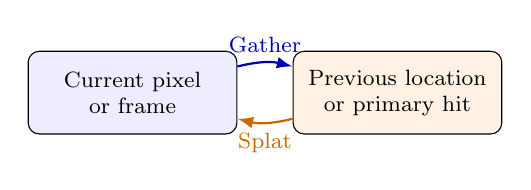
\begin{tikzpicture}[
    font=\footnotesize,
    frame/.style={draw,rounded corners,minimum width=2.65cm,minimum height=1.05cm,align=center},
    arr/.style={-{Latex[length=2mm]},thick},
    node distance=7mm
]
\node[frame,fill=blue!7] (current) {Current pixel\\or frame};
\node[frame,fill=orange!10,right=of current] (previous) {Previous location\\or primary hit};
\draw[arr,blue!70!black,bend left=14] (current) to node[above]{Gather} (previous);
\draw[arr,orange!80!black,bend left=14] (previous) to node[below]{Splat} (current);
\end{tikzpicture}
\caption{Gather performs backward lookup; splat performs forward projection.
The diagram explains correspondence direction and is not an empirical result.}
\label{fig:gather-splat}
\end{figure}

Gather-based reuse can provide a fallback for a newly revealed current pixel,
but its reprojected primary hit may be approximate. Reservoir Splatting
forwards the prior frame's exact primary hit into the current frame. A single
prior hit may splat to one current pixel, while multi-splatting projects at
several time samples to support motion blur. \method{ScatterBackup} combines
splatting with a gather fallback where no useful forward-splatted history
arrives. The evaluated renderer uses a reconnection shift after the primary
hit and therefore does not support delta materials in this configuration.

\section{System Design}

The extension deliberately avoids runtime mesh insertion and general rigid
body physics. The sphere and cube are created in a project-owned
\texttt{.pyscene} and initially placed outside the room. After scene load,
\texttt{Scene::findNodeIDByName()} locates the nodes. Each simulation update
uses \texttt{Scene::updateNodeTransform()}, triggering Falcor's existing scene
graph and acceleration-structure synchronization path.

\begin{figure}[t]
\centering
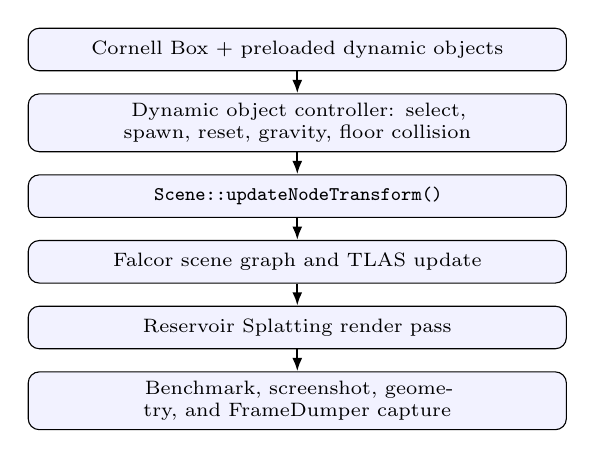
\begin{tikzpicture}[
    font=\scriptsize,
    box/.style={draw,rounded corners,fill=blue!5,text width=6.6cm,minimum height=5.4mm,align=center},
    arr/.style={-{Latex[length=1.7mm]},thick},
    node distance=2.8mm
]
\node[box] (scene) {Cornell Box + preloaded dynamic objects};
\node[box,below=of scene] (controller) {Dynamic object controller: select, spawn, reset, gravity, floor collision};
\node[box,below=of controller] (transform) {\texttt{Scene::updateNodeTransform()}};
\node[box,below=of transform] (tlas) {Falcor scene graph and TLAS update};
\node[box,below=of tlas] (render) {Reservoir Splatting render pass};
\node[box,below=of render] (capture) {Benchmark, screenshot, geometry, and FrameDumper capture};
\draw[arr] (scene)--(controller);
\draw[arr] (controller)--(transform);
\draw[arr] (transform)--(tlas);
\draw[arr] (tlas)--(render);
\draw[arr] (render)--(capture);
\end{tikzpicture}
\caption{System architecture of the interactive extension and capture
pipeline.}
\label{fig:architecture}
\end{figure}

The object controller exposes an object selector, editable spawn position,
spawn and reset actions, gravitational acceleration, and collision against one
horizontal floor plane. The sphere uses a rough metallic material and the cube
uses a rough plastic material. Both avoid delta materials.

The capture system separates renderer performance from output overhead. GPU
profiler measurements disable FrameDumper. Screenshot and video pipelines use
FrameDumper only when output is required. A separate geometry capture exports
world position, motion vectors, and validity masks to construct objective
disocclusion masks.

\section{Implementation}

The original repository provides the Reservoir Splatting render pass and its
temporal reuse modes. This project adds Linux build and runtime portability
fixes, Linux-compatible folder selection and FrameDumper behavior, deferred
readback, asynchronous PNG error handling, and Python capture hooks. It also
adds the dynamic Cornell Box scene, object controls, simplified physics,
automated renderer timing, deterministic camera-path capture, geometry
capture, high-sample references, masked error analysis, confidence intervals,
sensitivity analysis, and report figure generation.

\begin{table}[t]
\caption{Evaluated temporal configurations.}
\label{tab:modes}
\centering
\small
\begin{tabularx}{\columnwidth}{@{}lX@{}}
\toprule
Mode & Role in this report \\
\midrule
No temporal reuse & Runtime lower bound and noisy baseline \\
\method{GatherOnly + Robust} & Backprojection-based baseline \\
\method{ScatterOnly} & Single forward-splat configuration \\
\method{ScatterBackup} & Forward splat with gather fallback \\
\method{MultiSplatting} & Multi-time-sample splatting for motion blur \\
\bottomrule
\end{tabularx}
\end{table}

The high-sample experiment reports HDR normalized root mean squared error
(NRMSE), derived from MSE but normalized by reference RMS to make values
comparable across masked frames. It also reports log-luminance mean absolute
error (MAE), signed luminance bias, and non-finite pixel rate. FLIP is not used
because its result depends on a specified display transform and viewing
configuration; the present experiment instead evaluates linear HDR output and
log luminance directly.

\section{Experimental Design}

\subsection{Platform and Shared Settings}

\begin{table}[t]
\caption{Platform and shared settings.}
\label{tab:setup}
\centering
\small
\begin{tabularx}{\columnwidth}{@{}lX@{}}
\toprule
Variable & Value \\
\midrule
GPU & NVIDIA GeForce RTX 5070 Ti, 16 GB \\
Driver & NVIDIA 595.58.03 \\
OS & Arch Linux \\
API / framework & Vulkan / Falcor 8 \cite{falcor} \\
Resolution & $960{\times}540$ \\
Samples per pixel & 1 for evaluated modes \\
Spatial resampling & Enabled \\
\bottomrule
\end{tabularx}
\end{table}

All comparisons use the same scene, rendering settings, object trajectory or
camera path, and resolution within their experiment. FrameDumper is disabled
for renderer-only GPU timing.

\subsection{Falling-Sphere Experiment}

The falling-sphere experiment uses a rough metallic sphere, a shutter speed of
0.05\,s, and two multi-splat time partitions. GPU timings contain 68 valid
profiler frames from one falling sequence per mode. Representative images use
falling-sphere frame 32. The experiment asks how much GPU time each
configuration requires during object motion and what visible differences
appear in a controlled representative frame. Frame-to-frame standard
deviations are not confidence intervals across independent benchmark runs.

\subsection{Reference-Based Camera Disocclusion}

The objective quality experiment isolates newly revealed surfaces from motion
blur by setting shutter speed to zero. Three modes follow an identical
90-frame horizontal camera path: \method{GatherOnly + Robust},
\method{ScatterOnly}, and \method{ScatterBackup}. Each mode has five
independent initial seeds, and ten target frames are evaluated.

For each target frame, two independent references accumulate 1024 one-sample
frames. Their average is the high-sample reference, and their difference
estimates the reference noise floor. A current pixel is marked disoccluded
when its motion-vector-reprojected coordinate is outside the previous frame,
maps to no previous geometry, or has a previous world position differing from
the current world position by more than 0.02 scene units. The mask is dilated
by one pixel to include immediate boundary behavior. Thresholds 0.01 and 0.04
are also analyzed.

Metrics are computed only inside this mask: HDR RGB NRMSE, log-luminance MAE,
signed luminance bias, masked and full-frame non-finite pixel rates, and paired
95\% confidence intervals over five independent seeds.

\section{Performance Results}

\begin{figure*}[t]
\centering
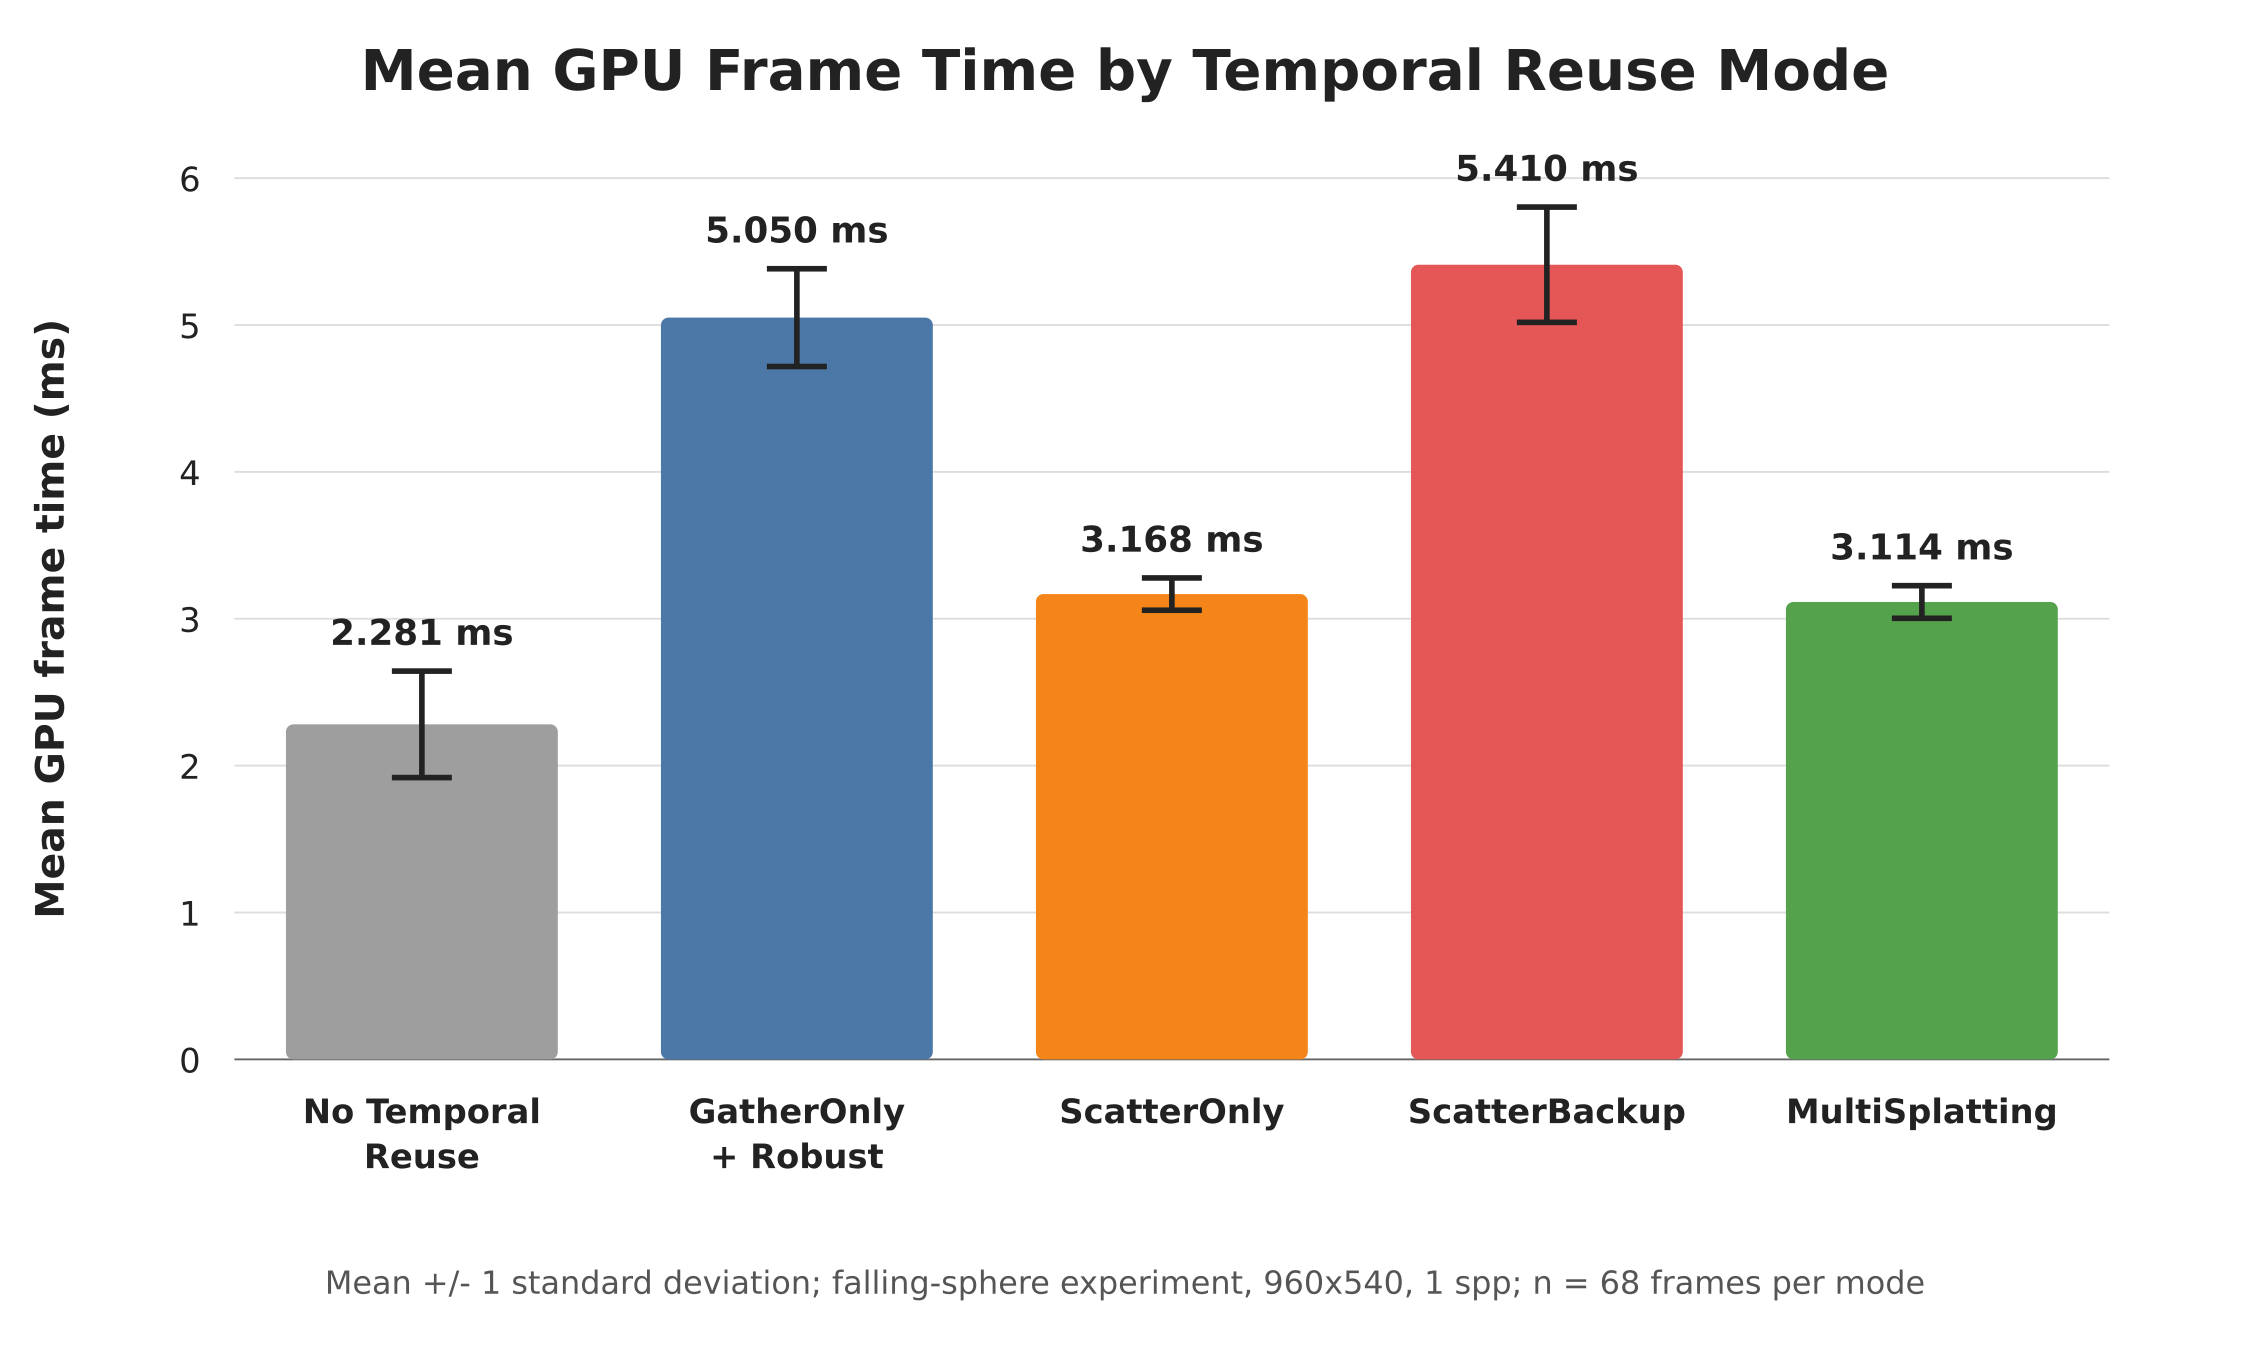
\includegraphics[width=.76\textwidth]{dynamic-object-gpu-frame-time.png}
\caption{Mean GPU frame time with one-standard-deviation error bars for one
falling-sphere sequence at $960{\times}540$ and 1 spp. Runtime alone does not
establish image quality.}
\label{fig:gpu-time}
\end{figure*}

\begin{table}[t]
\caption{GPU profiler results over 68 falling-sphere frames. Times are in ms.}
\label{tab:timing}
\centering
\small
\setlength{\tabcolsep}{3.4pt}
\begin{tabular}{@{}lrrrr@{}}
\toprule
Mode & Mean & Std. & Min & Max \\
\midrule
No reuse & 2.281 & 0.362 & 2.129 & 4.436 \\
Gather robust & 5.050 & 0.333 & 2.494 & 5.363 \\
Scatter only & 3.168 & 0.110 & 2.293 & 3.258 \\
Scatter backup & 5.410 & 0.392 & 2.225 & 5.577 \\
Multi-splatting & 3.114 & 0.111 & 2.233 & 3.221 \\
\bottomrule
\end{tabular}
\end{table}

No temporal reuse is the fastest configuration, but its representative image
is visibly noisier. \method{ScatterOnly} and \method{MultiSplatting} have
similar measured cost and are substantially less expensive than
\method{GatherOnly + Robust} and \method{ScatterBackup}.
\method{ScatterBackup} is the most expensive tested configuration because it
combines forward splatting with backup reuse.

FrameDumper overhead was measured separately. \method{MultiSplatting} with PAM
output recorded 69 frames at a mean wall-frame time of 9.503\,ms
(105.23 FPS). This includes readback and file output and is not directly
comparable to renderer-only GPU timings.

\section{Visual and Reference-Based Results}

\begin{figure*}[t]
\centering
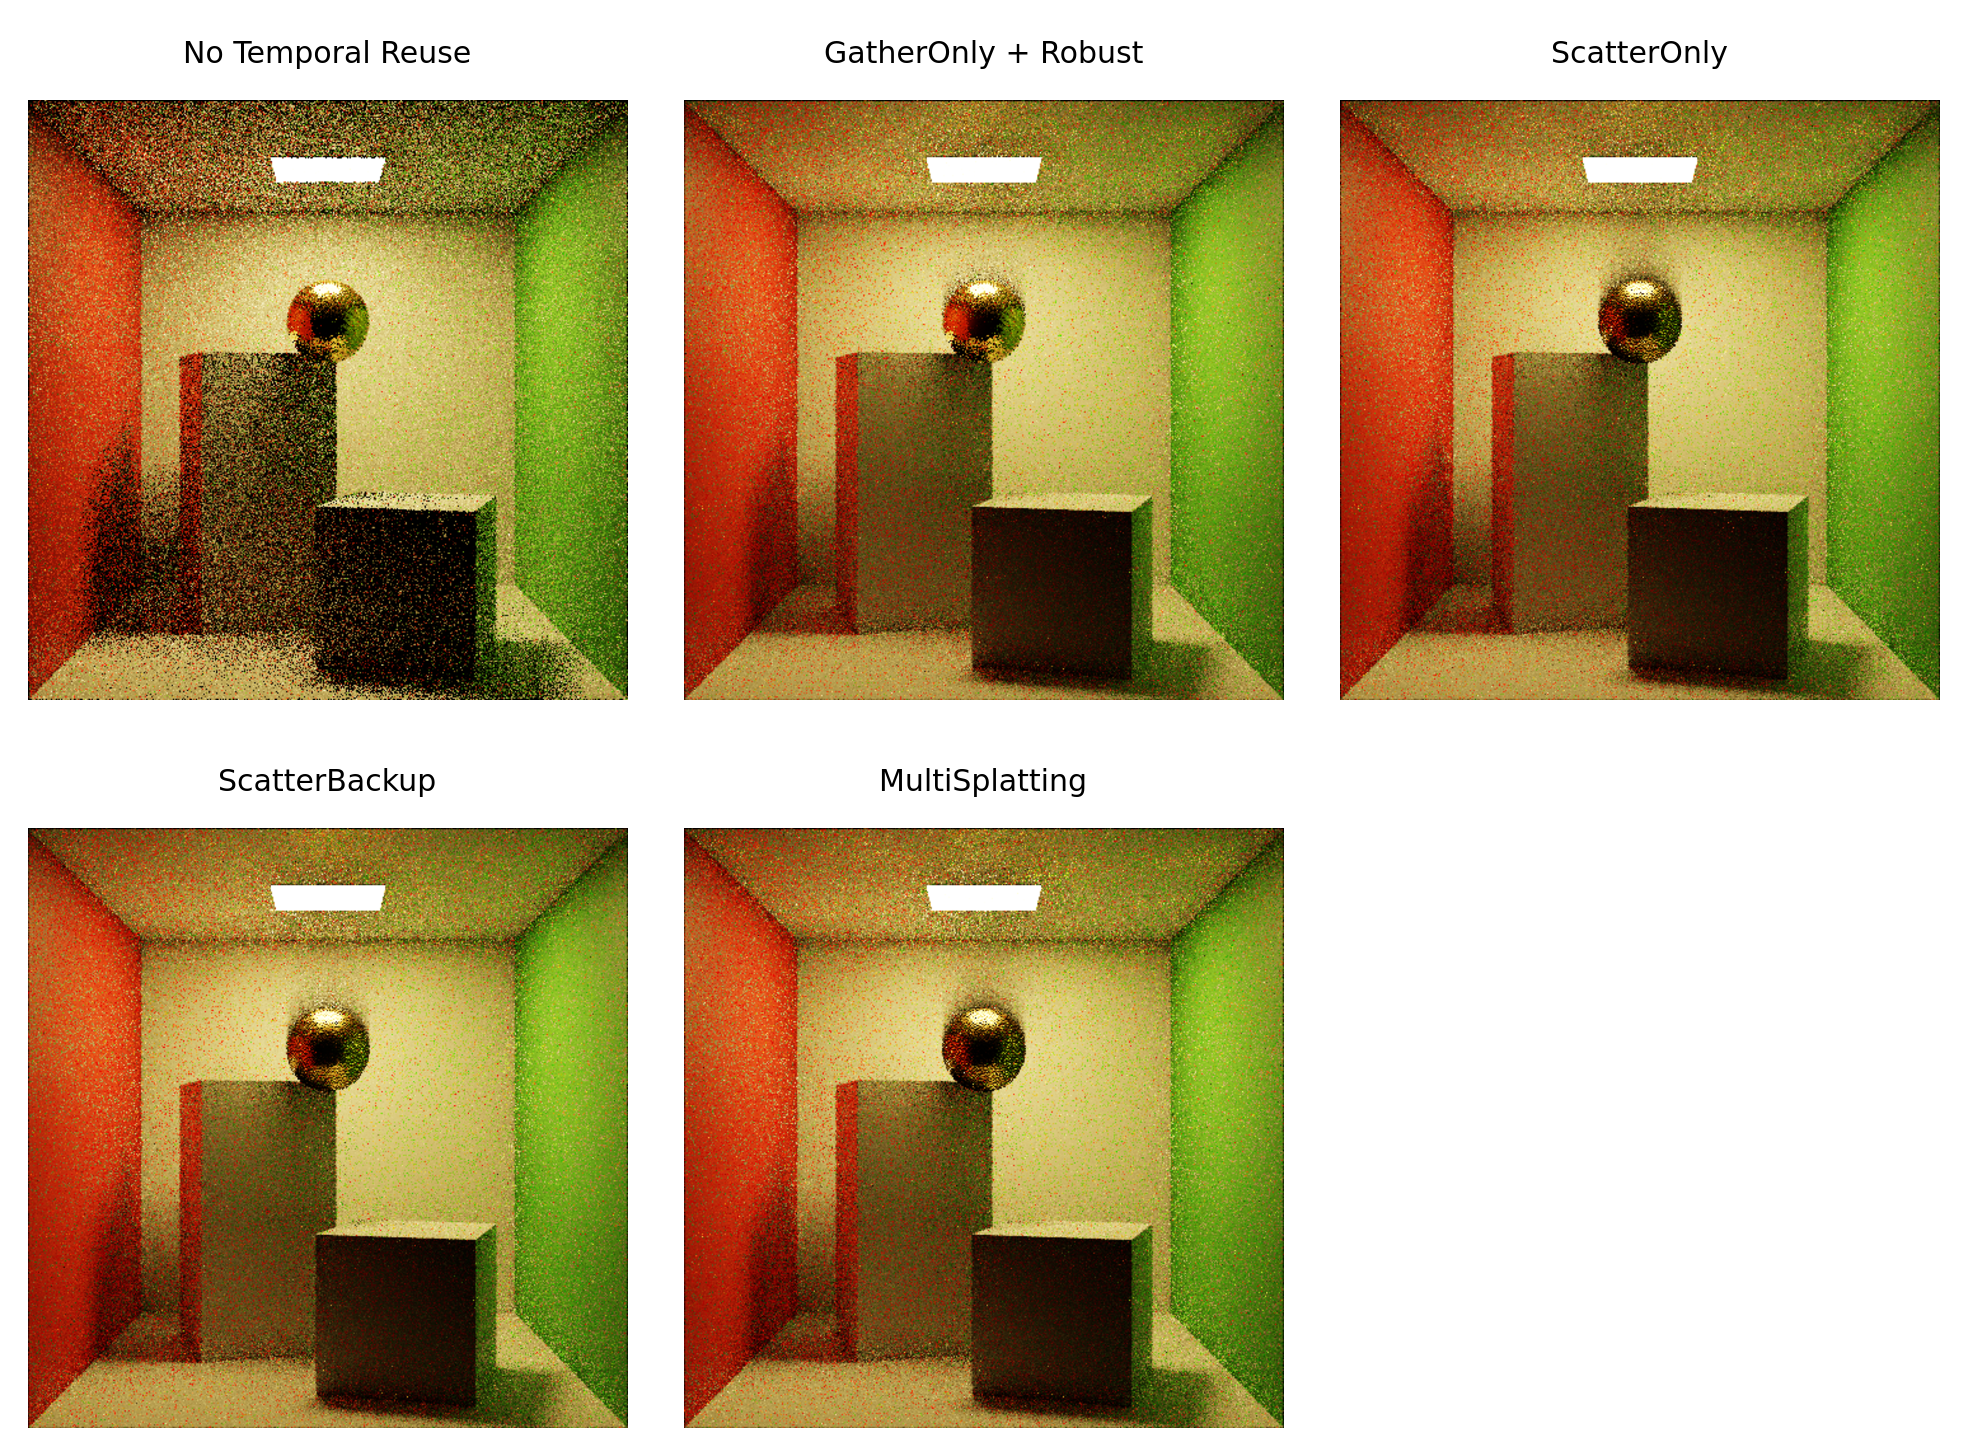
\includegraphics[width=\textwidth]{dynamic-object-five-mode-comparison.png}
\caption{Representative falling-sphere frame at 1 spp. No temporal reuse
exhibits substantially stronger high-frequency noise. This qualitative
single-frame comparison cannot rank accuracy or temporal stability.}
\label{fig:five-mode}
\end{figure*}

\begin{figure*}[t]
\centering
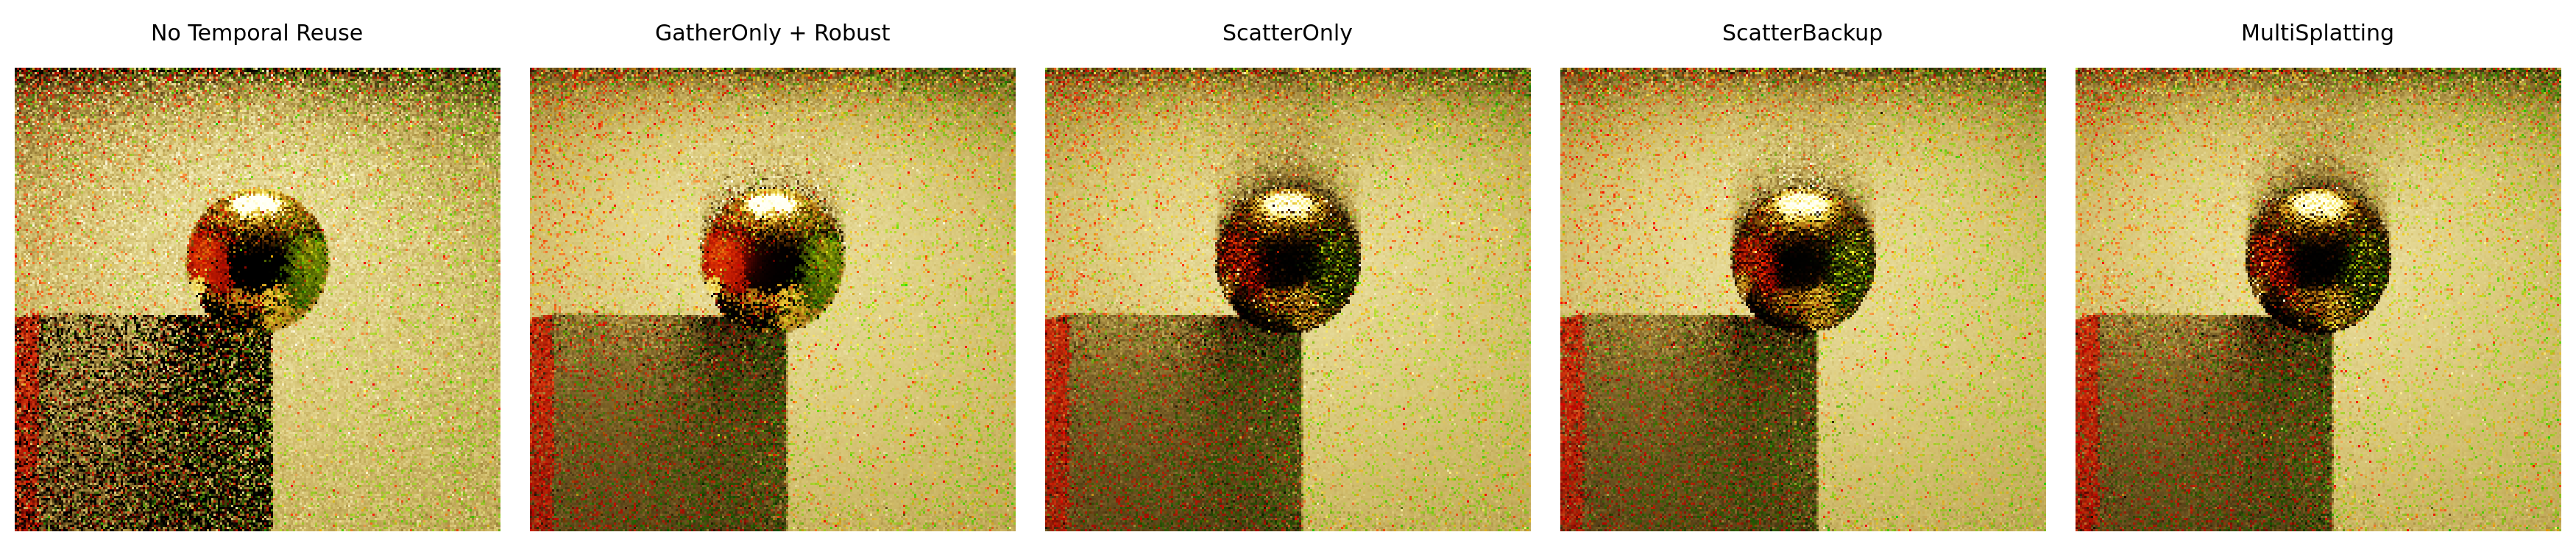
\includegraphics[width=.94\textwidth]{dynamic-object-detail-crops.png}
\caption{Enlarged crops emphasizing the moving sphere, its boundary, and a
newly revealed region. The crops identify useful inspection areas but do not
provide an accuracy ranking without a matching reference.}
\label{fig:crops}
\end{figure*}

Figures~\ref{fig:five-mode} and \ref{fig:crops} show that disabling temporal
reuse produces substantially stronger high-frequency noise at 1 spp. The
moving sphere boundary and newly revealed region provide useful locations for
qualitative inspection. A single image without a reference cannot rank the
accuracy or temporal stability of the reuse modes.

\begin{figure*}[t]
\centering
\begin{subfigure}[t]{.48\textwidth}
\centering
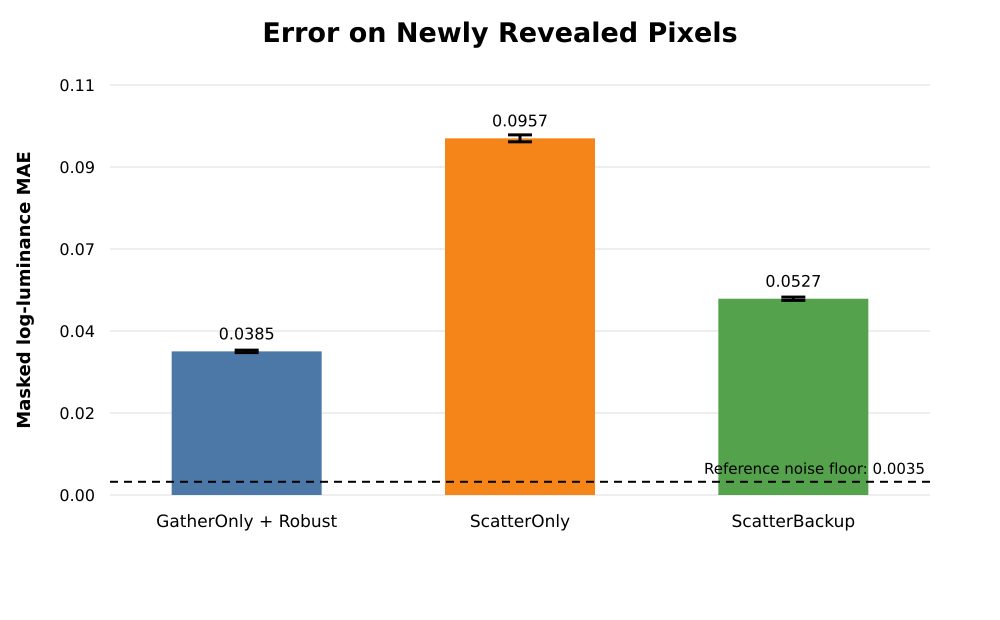
\includegraphics[width=\linewidth]{disocclusion-error-summary.png}
\caption{Aggregate masked log-luminance MAE with paired-seed uncertainty and
the measured reference noise floor.}
\label{fig:disocclusion-summary}
\end{subfigure}
\hfill
\begin{subfigure}[t]{.48\textwidth}
\centering
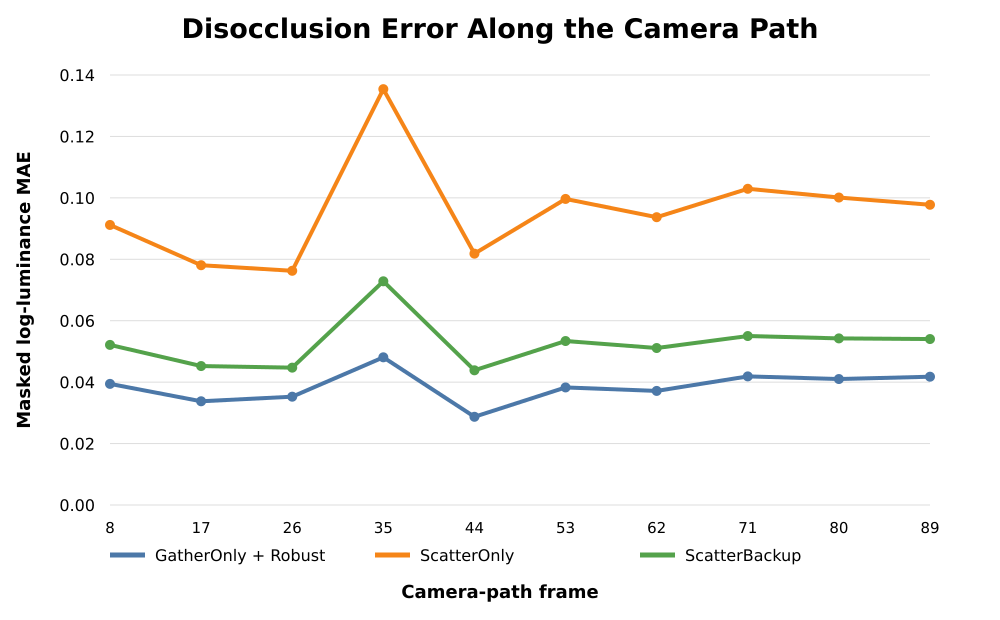
\includegraphics[width=\linewidth]{disocclusion-error-over-time.png}
\caption{Masked error at sampled frames along the controlled camera path.}
\label{fig:disocclusion-time}
\end{subfigure}
\caption{Reference-based error on newly revealed pixels. Robust gather has
the lowest error in this camera-disocclusion experiment; the conclusion does
not rank full-frame or motion-blur quality.}
\label{fig:disocclusion}
\end{figure*}

\begin{table}[t]
\caption{Reference-based error inside the disocclusion mask.}
\label{tab:quality}
\centering
\small
\begin{tabular}{@{}lrr@{}}
\toprule
Method & HDR NRMSE & Log-luma MAE \\
\midrule
Gather robust & 0.4774 & 0.0385 \\
Scatter only & 0.8728 & 0.0957 \\
Scatter backup & 0.5965 & 0.0527 \\
\bottomrule
\end{tabular}
\end{table}

The mean reference noise floor is approximately 0.0278 NRMSE and 0.0035
log-luminance MAE. All test and reference outputs contain zero non-finite
pixels. Paired seed-level comparisons show separated confidence intervals:
Gather has 0.0572 lower log-luminance MAE than \method{ScatterOnly}
(95\% CI $[0.0562,0.0581]$) and 0.0141 lower error than
\method{ScatterBackup} (95\% CI $[0.0135,0.0147]$).
\method{ScatterBackup} has 0.0430 lower error than \method{ScatterOnly}
(95\% CI $[0.0424,0.0437]$).

The ranking remains unchanged at world-position thresholds 0.01, 0.02, and
0.04. For this controlled camera pan, robust gather therefore produces the
lowest reference error on immediately newly revealed pixels.
\method{ScatterBackup}'s improvement over \method{ScatterOnly} confirms the
value of a gather fallback when no useful forward-splatted history exists.

\begin{figure*}[t]
\centering
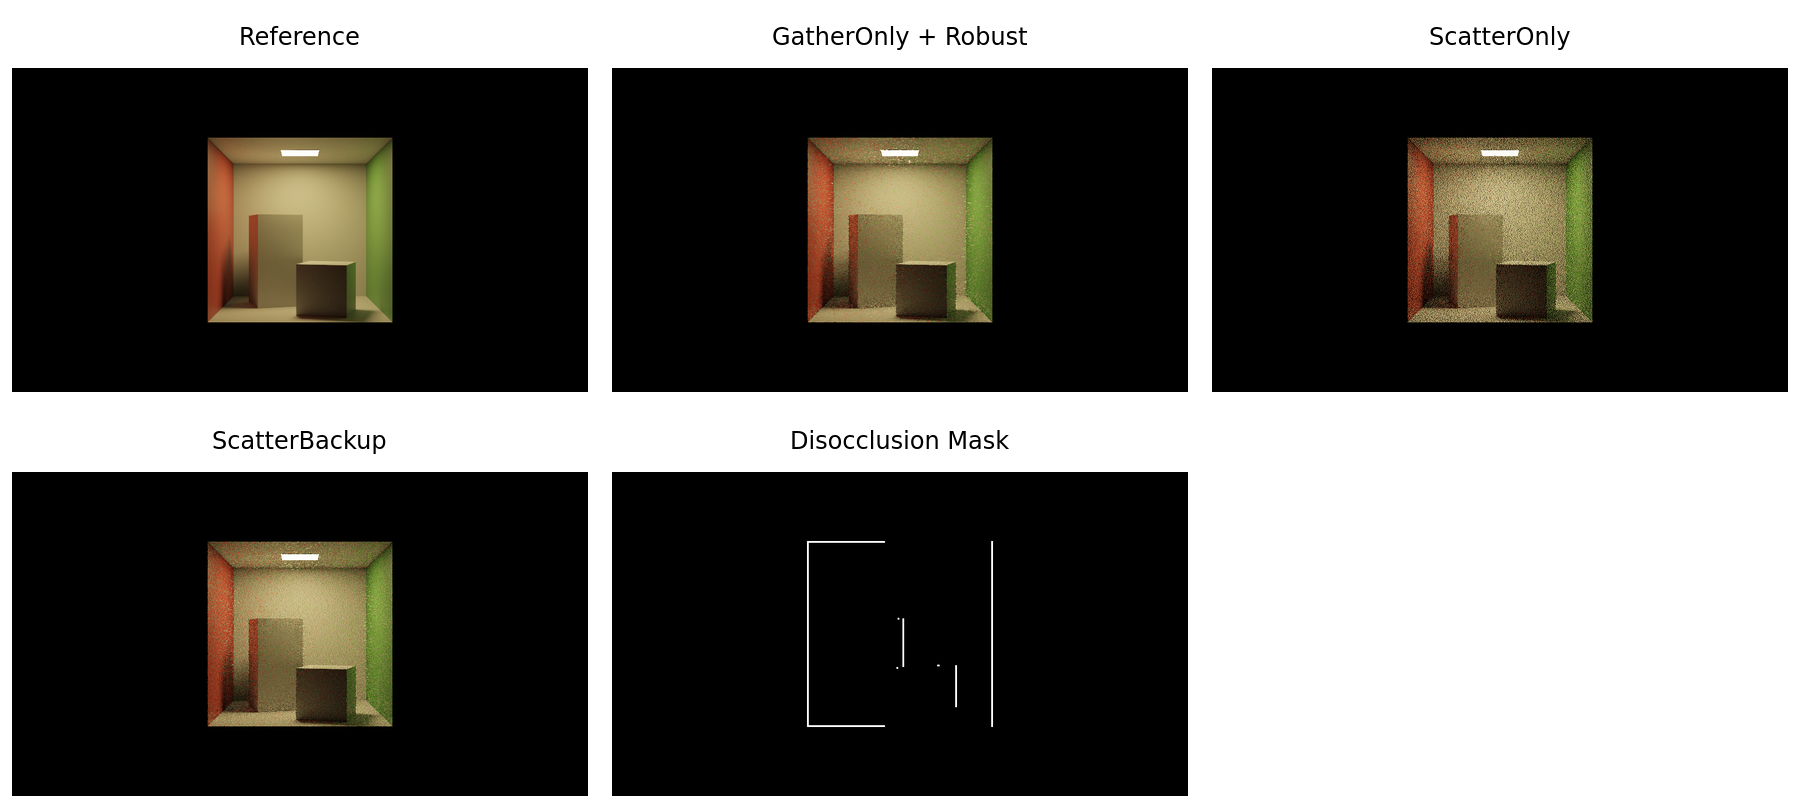
\includegraphics[width=.94\textwidth]{disocclusion-representative-frame-44.png}
\caption{Illustrative target frame 44: high-sample reference, three evaluated
methods, and the objective disocclusion mask. This frame shows what is
measured; the aggregate ranking comes from all target frames and seeds.}
\label{fig:reference-frame}
\end{figure*}

This result does not contradict the motivation for splatting. A newly revealed
pixel has no corresponding previous-frame primary hit to forward splat, so
\method{ScatterOnly} is expected to be weak in this specific region. The
result does not establish that gather has the best full-frame quality,
temporal stability outside the mask, dynamic-object behavior, or motion-blur
quality.

\section{Limitations and Future Work}

The interactive demo contains only a preloaded sphere and cube. Its simplified
simulation omits rotation, stacking, and object-to-object collision and uses
one floor collision plane. Delta materials, glass, and caustics are outside
the evaluated renderer configuration. GPU timing uses one falling sequence
per mode rather than repeated benchmark runs. The objective experiment
evaluates camera-driven disocclusion in one Cornell Box path, not
moving-object disocclusion or motion blur. It uses HDR NRMSE and
log-luminance MAE rather than display-referred FLIP, and the tested scene and
resolution range is limited.

Future work should capture high-sample references for moving-object
disocclusion and nonzero shutter speed, add display-referred FLIP with a
documented tone mapper and viewing setup, repeat GPU timing across independent
runs, and evaluate more scenes, object velocities, shutter speeds, and
resolutions. Engineering extensions include rigid-body rotation, collision
response, runtime asset import, and a compatible ReSTIR BDPT approach for
delta materials and caustics.

\section{Conclusion}

This project successfully reproduces the official Reservoir Splatting renderer
on an Arch Linux RTX 5070 Ti system and extends it with an interactive dynamic
geometry demonstration. The extension uses existing Falcor node-transform and
acceleration-structure update paths, and its scripts provide reproducible
renderer benchmarks, image captures, video captures, geometry masks, and
high-sample references.

The measured results expose a meaningful tradeoff. \method{ScatterOnly} and
\method{MultiSplatting} are less expensive than robust gather and backup
configurations in the falling-sphere benchmark, while temporal reuse visibly
reduces noise relative to disabling reuse. In a targeted camera-disocclusion
experiment, robust gather is most accurate on newly revealed pixels and
\method{ScatterBackup} substantially improves over \method{ScatterOnly}.
Temporal reuse methods must therefore be evaluated against the visibility
event and quality criterion they are intended to handle, rather than ranked by
frame time or one representative image alone.

\begin{thebibliography}{9}
\bibitem{reservoir-splatting}
J. Liu, D. Lin, M. Kettunen, C. Wyman, and R. Ramamoorthi,
``Reservoir Splatting for Temporal Path Resampling and Motion Blur,''
\emph{ACM SIGGRAPH Conference Proceedings}, 2025.

\bibitem{gris}
D. Lin et al.,
``Generalized Resampled Importance Sampling: Foundations of ReSTIR,''
\emph{ACM SIGGRAPH Conference Proceedings}, 2022.

\bibitem{area-restir}
S. Zhang et al.,
``Area ReSTIR: Resampling for Real-Time Defocus and Antialiasing,''
\emph{ACM SIGGRAPH Asia Conference Proceedings}, 2024.

\bibitem{falcor}
NVIDIA,
``Falcor: Real-Time Rendering Framework,'' version 8,
\url{https://github.com/NVIDIAGameWorks/Falcor}.
\end{thebibliography}

\end{document}
